%\title{Project Report}
%
%%% Preamble
\documentclass[paper=a4, fontsize=11pt]{scrartcl}
\usepackage[T1]{fontenc}
\usepackage{fourier}

\usepackage[english]{babel}															% English language/hyphenation
\usepackage[protrusion=true,expansion=true]{microtype}	
\usepackage{amsmath,amsfonts,amsthm} % Math packages
\usepackage[pdftex]{graphicx}	
\usepackage{url}
\usepackage{hyperref}
\usepackage{graphicx}
\usepackage{wrapfig}
\usepackage[margin=0.75in]{geometry}

%%% Custom sectioning
\usepackage{sectsty}
\allsectionsfont{\centering \normalfont\scshape}


%%% Custom headers/footers (fancyhdr package)
\usepackage{fancyhdr}
\pagestyle{fancyplain}
\fancyhead{}											% No page header
\fancyfoot[L]{}											% Empty 
\fancyfoot[C]{}											% Empty
\fancyfoot[R]{\thepage}									% Pagenumbering
\renewcommand{\headrulewidth}{0pt}			% Remove header underlines
\renewcommand{\footrulewidth}{0pt}				% Remove footer underlines
\setlength{\headheight}{3.6pt}
\date{}


%%% Equation and float numbering
\numberwithin{equation}{section}		% Equationnumbering: section.eq#
\numberwithin{figure}{section}			% Figurenumbering: section.fig#
\numberwithin{table}{section}				% Tablenumbering: section.tab#


%%% Maketitle metadata
\newcommand{\horrule}[1]{\rule{\linewidth}{#1}} 	% Horizontal rule

\title{
		\vspace{-0.5in} 	
		\usefont{OT1}{bch}{b}{n}
		\normalfont \normalsize \textsc{Durham Computer Science} \\ [5pt]
		\horrule{0.5pt} \\[0.4cm]
		\huge Machine Learning Assignment - LLLL76\\
		\horrule{2pt} \\[0.5cm]
		\vspace{-1in} 	
}

%%% Begin document
\begin{document}
\maketitle
\section{Discussion/details of approaches chosen and experimental procedure}

\subsection{kNN and Variations}

K nearest neighbours was implemented and tested first. The benefits of kNN is that is is very fast to train only needing the time taken to plot all train data. The disadvantages of kNN is the slow query time, this is due to slow look up in high dimensional space. There is only a single value that can be changed in basic kNN to alter its behaviour, the number of neighbours that are used, k. There are a few more advancements on kNN based around the weighting of the neighbours. The weighting cane be done based on the inverse square of the distance between the query and its neighbour or the similarity between the query and its neighbour, both of which have been implemented.

\subsection{SVM}

Support Vector Machines are based around the idea of a linear separator, that any two classes can be split by a line, and to find the best line there should be a maximum separating margin. The implementation of this approach has a significant number of variables, kernel, degree, C, gamma and the class weighting.

\subsection{Experimental Procedure}

Different data splits were implemented, each was used to test the three different kNN implementations. A grid search was performed on all three implementations of kNN a k value of one to one hundred was used with the data from one to ten being shown in the tables bellow. An external library was used to perform a grid search on SVM, this performed SVM with different kernals, gamma, degree and C values, then returned the percentage of correct tests. Any results taken are averages of ten runs of those values, this includes accuracy, precision, recall and F1 score.

\section{Evidence of the performance of your chosen approaches on the data}

\subsection{Percentages}

\begin{tabular}{ |p{2cm}||p{4cm}|p{4cm}|p{4cm}| }
 \hline
 \multicolumn{4}{|c|}{kNN Results} \\
 \hline
K Value & kNN - 70:30 & kNN - 80:20 & kNN - 90:10\\
 \hline
1 & 95.14 & 95.41 & 95.93 \\
2 & 93.51 & 92.97 & 93.14 \\
3 & 95.01 & 95.30 & 95.27 \\
4 & 94.35 & 93.79 & 94.43 \\
5 & 94.99 & 95.24 & 95.64 \\
6 & 94.37 & 94.17 & 94.81 \\
7 & 94.50 & 94.99 & 95.49 \\
8 & 94.25 & 94.43 & 94.23 \\
9 & 94.64 & 94.59 & 94.83 \\
10 & 94.01 & 93.95 & 94.26 \\
 \hline
 Best & 1 - 95.14 & 1 - 95.41 & 1 - 95.93 \\
 \hline
\end{tabular}
\\
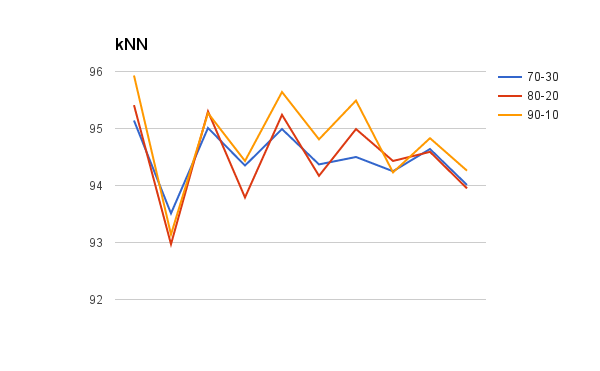
\includegraphics[width=\textwidth]{knn.png}
\\

\begin{tabular}{ |p{2cm}||p{4cm}|p{4cm}|p{4cm}| }
 \hline
 \multicolumn{4}{|c|}{kNN Weighted Inverse Results} \\
 \hline
K Value & kNN Weighted Inverse - 70:30 & kNN Weighted Inverse - 80:20 & kNN Weighted Inverse - 90:10\\
 \hline
1 & 95.04 & 95.29 & 95.60 \\
2 & 95.04 & 95.24 & 95.94 \\
3 & 95.36 & 95.60 & 95.69 \\
4 & 95.47 & 95.74 & 96.18 \\
5 & 95.70 & 95.79 & 96.14 \\
6 & 95.65 & 95.93 & 96.17 \\
7 & 95.59 & 96.00 & 96.24 \\
8 & 95.34 & 95.95 & 96.28 \\
9 & 95.25 & 95.89 & 96.17 \\
10 & 95.20 & 95.35 & 95.49 \\
 \hline
 Best & 5 - 95.70 & 7 - 96.00 & 8 - 96.28 \\
 \hline
\end{tabular}
\\
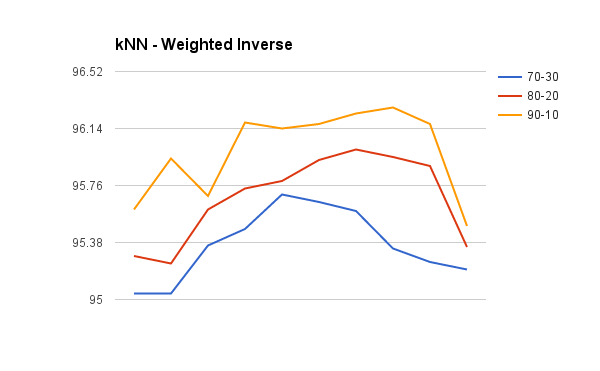
\includegraphics[width=\textwidth]{knninverse.png}
\\

\begin{tabular}{ |p{2cm}||p{4cm}|p{4cm}|p{4cm}| }
 \hline
 \multicolumn{4}{|c|}{kNN Weighted Similarity Results} \\
 \hline
K Value & kNN Weighted Similarity - 70:30 & kNN Weighted Similarity - 80:20 & kNN Weighted Similarity - 90:10\\
 \hline
1 & 94.97 & 95.19 & 95.71 \\
2 & 92.58 & 92.80 & 93.22 \\
3 & 95.23 & 95.68 & 95.63 \\
4 & 93.78 & 94.13 & 93.81 \\
5 & 94.82 & 95.08 & 95.37 \\
6 & 93.69 & 94.17 & 94.43 \\
7 & 94.59 & 94.85 & 95.00 \\
8 & 93.73 & 94.14 & 94.80 \\
9 & 94.50 & 94.58 & 94.91 \\
10 & 93.57 & 94.11 & 94.59 \\
 \hline
 Best & 3 - 95.23 & 3 - 95.68 & 1 - 95.71 \\
 \hline
\end{tabular}
\\
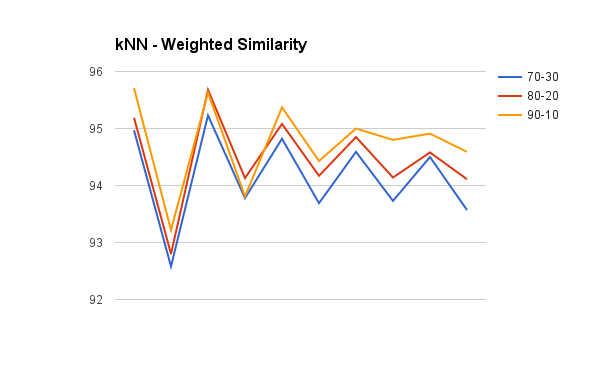
\includegraphics[width=\textwidth]{knnsimilar.png}
\\

\begin{tabular}{ |p{2cm}|p{2cm}|p{2cm}|p{2cm}||p{4cm}| }
 \hline
 \multicolumn{5}{|c|}{SVM} \\
 \hline
Kernal & C Value & Gamma & Degree & Result\\
 \hline
RBF & 100 & 0.01 & - & 98.08 \\
LINEAR & 1 & - & - & 96.31 \\
POLY & 1 & 0.1 & 5 & 97.63 \\
SIGMOID & 1000 & 0.001 & - & 96.8 \\
 \hline
\end{tabular}
\\
\\
\\
The best from each table are:\\
- kNN - 90:10 train:test, where K = 1 with 95.93\% accuracy \\
- kNN Weighted Inverse - 90:10 train:test, where K = 8 with 96.28\% accuracy \\
- kNN Weighted Similarity - 90:10 train:test, where K = 1 with 95.71\% accuracy \\
- SVM using the RBF kernal with C = 100 and Gamma = 0.01 with 98.08\% accuracy

\subsection{Accuracy, Precision, Recall and F-Measure}

- kNN - 90:10 train:test, where K = 1\\
Accuracy: 0.959706959707\\
Precision: 0.959706959707\\
Recall: 0.959706959707\\
F1: 0.959706959707\\
\\
- kNN Weighted Inverse - 90:10 train:test, where K = 8\\
Accuracy: 0.951465201465\\
Precision: 0.951465201465\\
Recall: 0.951465201465\\
F1: 0.951465201465\\
\\
- kNN Weighted Similarity - 90:10 train:test, where K = 1\\
Accuracy: 0.957875457875\\
Precision: 0.957875457875\\
Recall: 0.957875457875\\
F1: 0.957875457875\\
\\
- SVM using the RBF kernal with C = 100 and Gamma = 0.01\\
Accuracy: 0.981391092129\\
Precision: 0.981391092129\\
Recall: 0.981391092129\\
F1: 0.981391092129

\subsection{Confusion Matrix}

\subsubsection{kNN - 90:10 train:test, where K = 1}
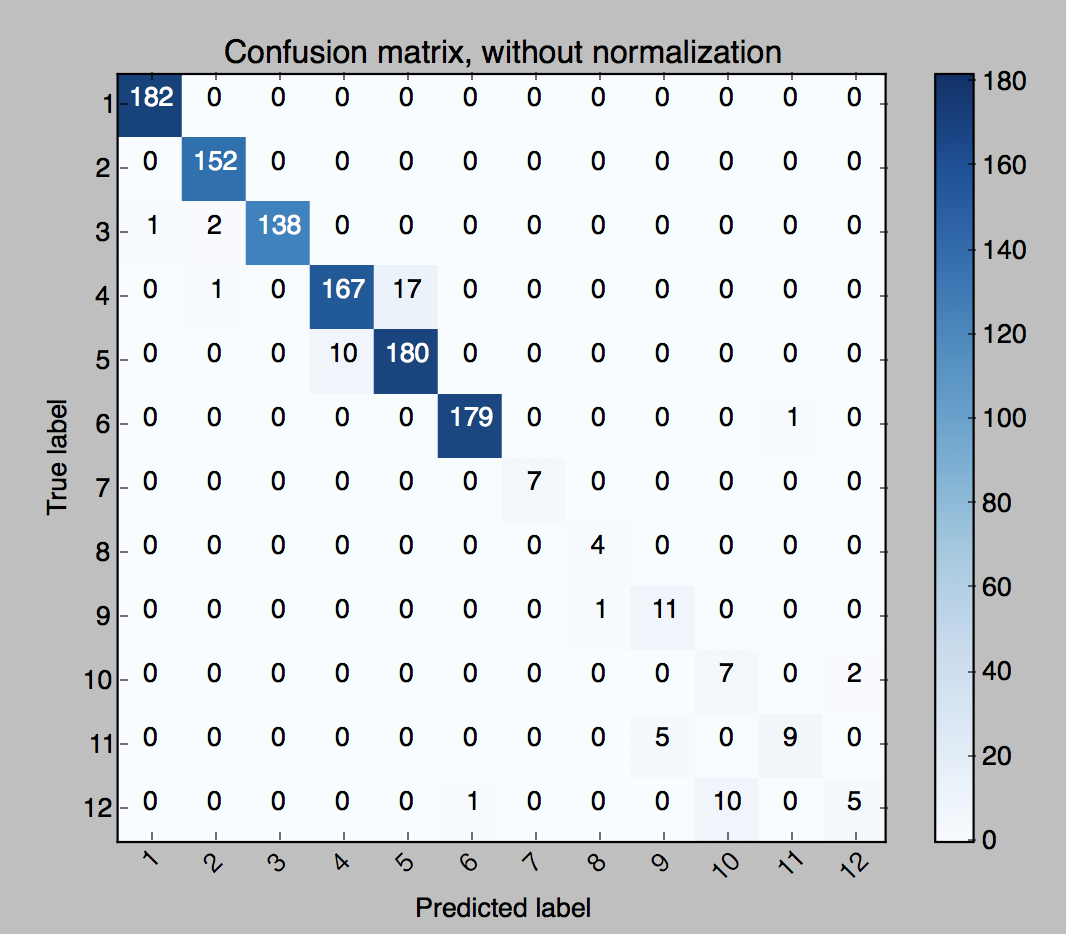
\includegraphics[width=0.5\textwidth]{first.png}
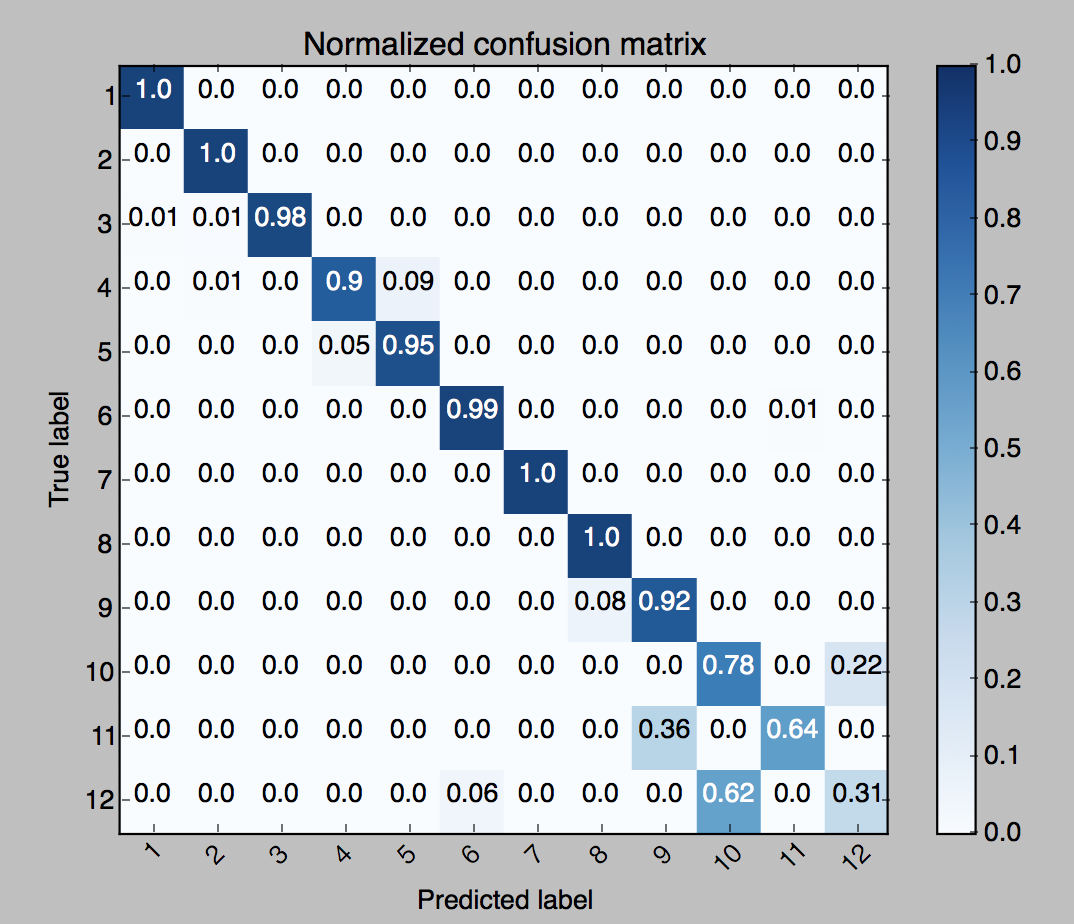
\includegraphics[width=0.5\textwidth]{firstN.png}
\\
\\
\subsubsection{kNN Weighted Inverse - 90:10 train:test, where K = 8}
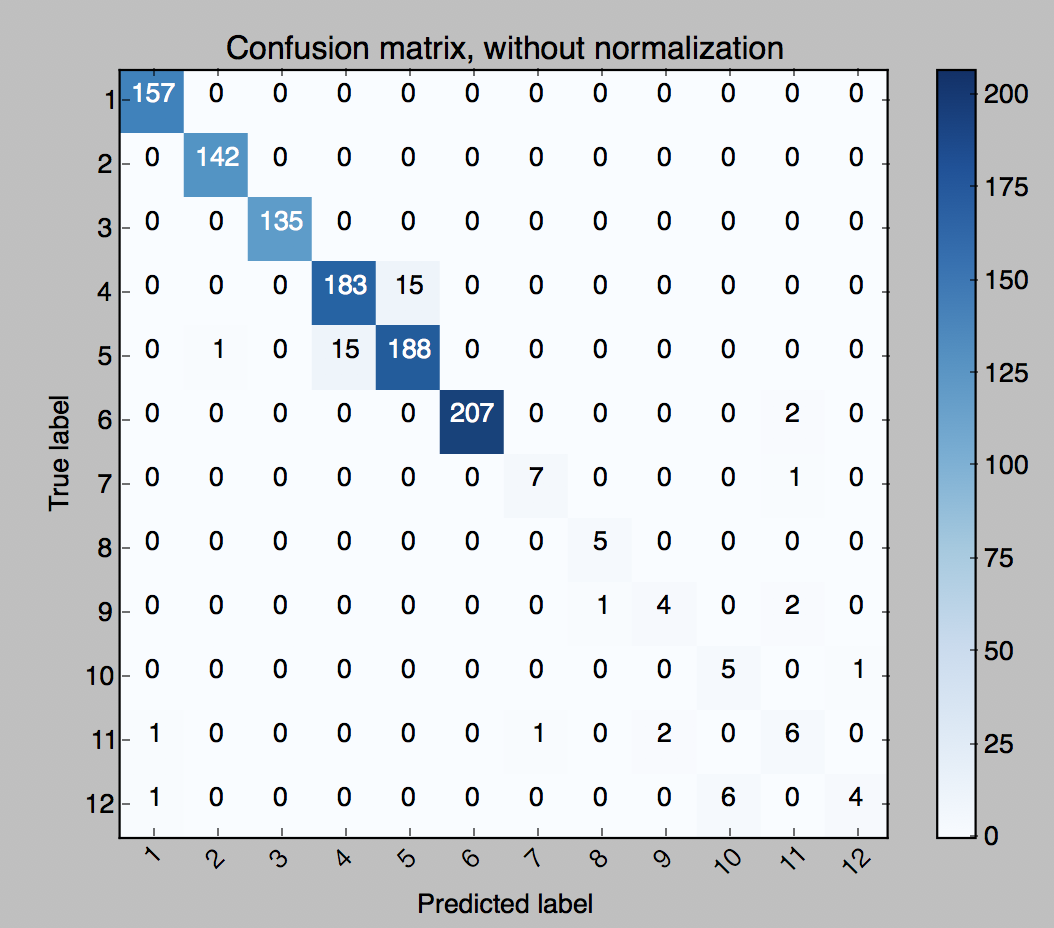
\includegraphics[width=0.5\textwidth]{second.png}
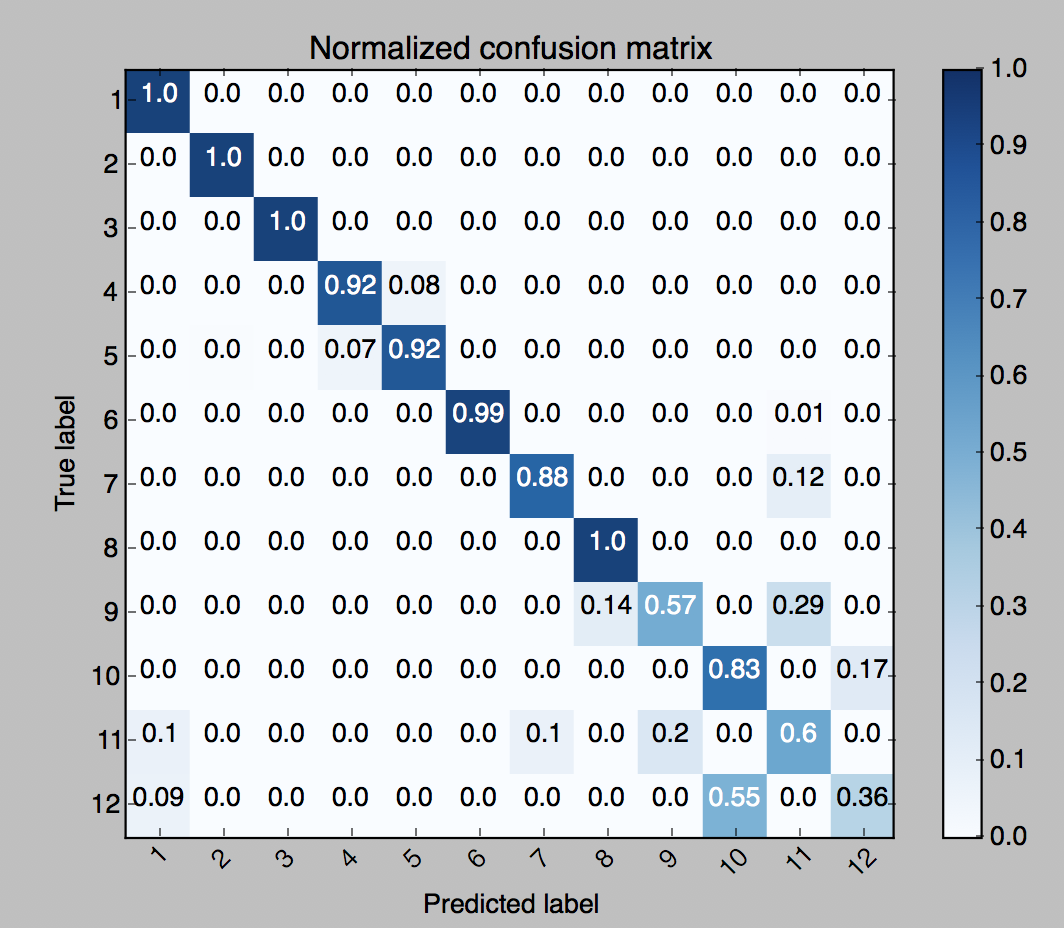
\includegraphics[width=0.5\textwidth]{secondN.png}
\\
\\
\subsubsection{kNN Weighted Similarity - 90:10 train:test, where K = 1}
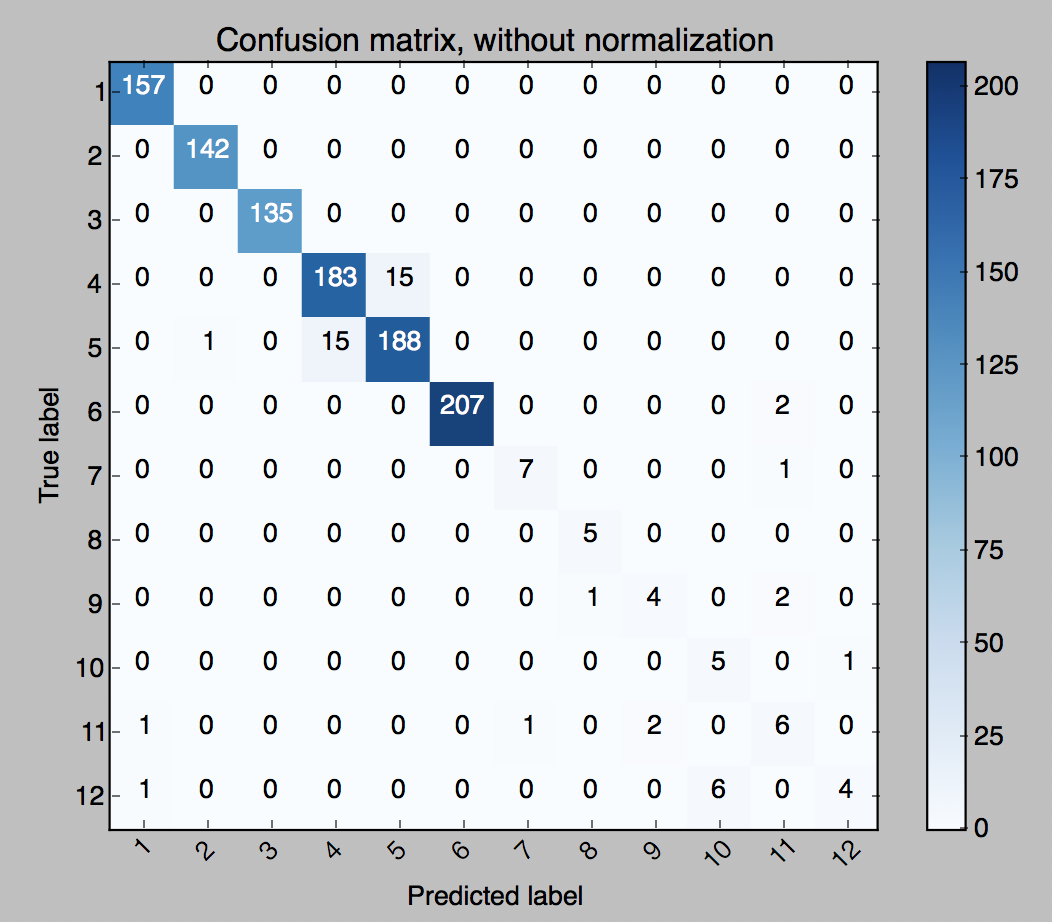
\includegraphics[width=0.5\textwidth]{third.png}
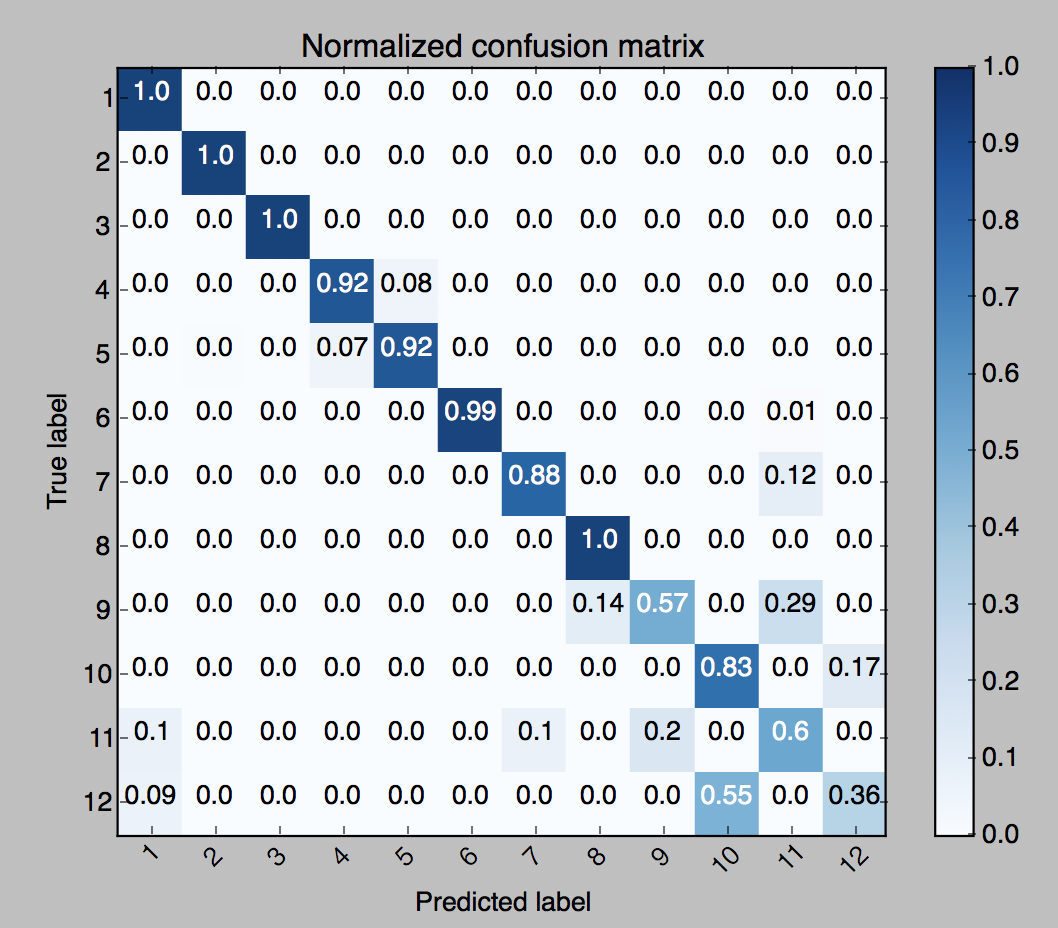
\includegraphics[width=0.5\textwidth]{thirdN.png}
\\
\\
\subsubsection{SVM using the RBF kernal with C = 100 and Gamma = 0.01}
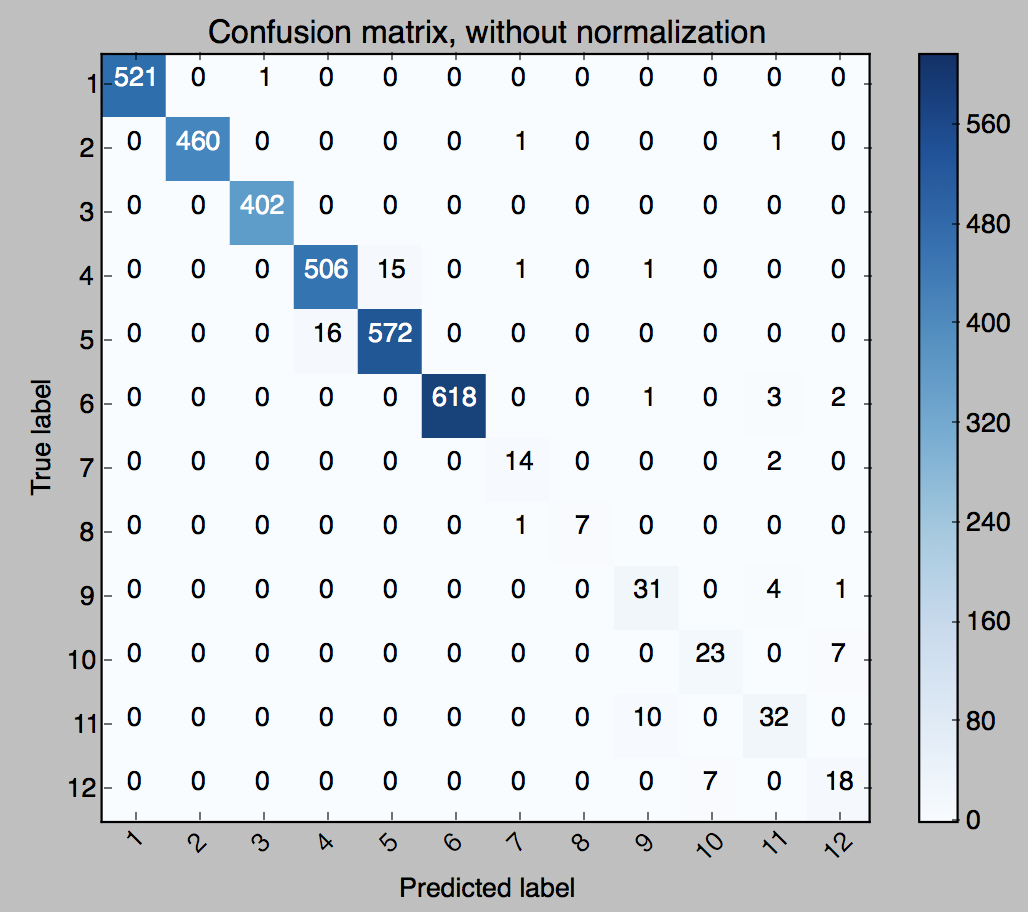
\includegraphics[width=0.5\textwidth]{fourth.png}
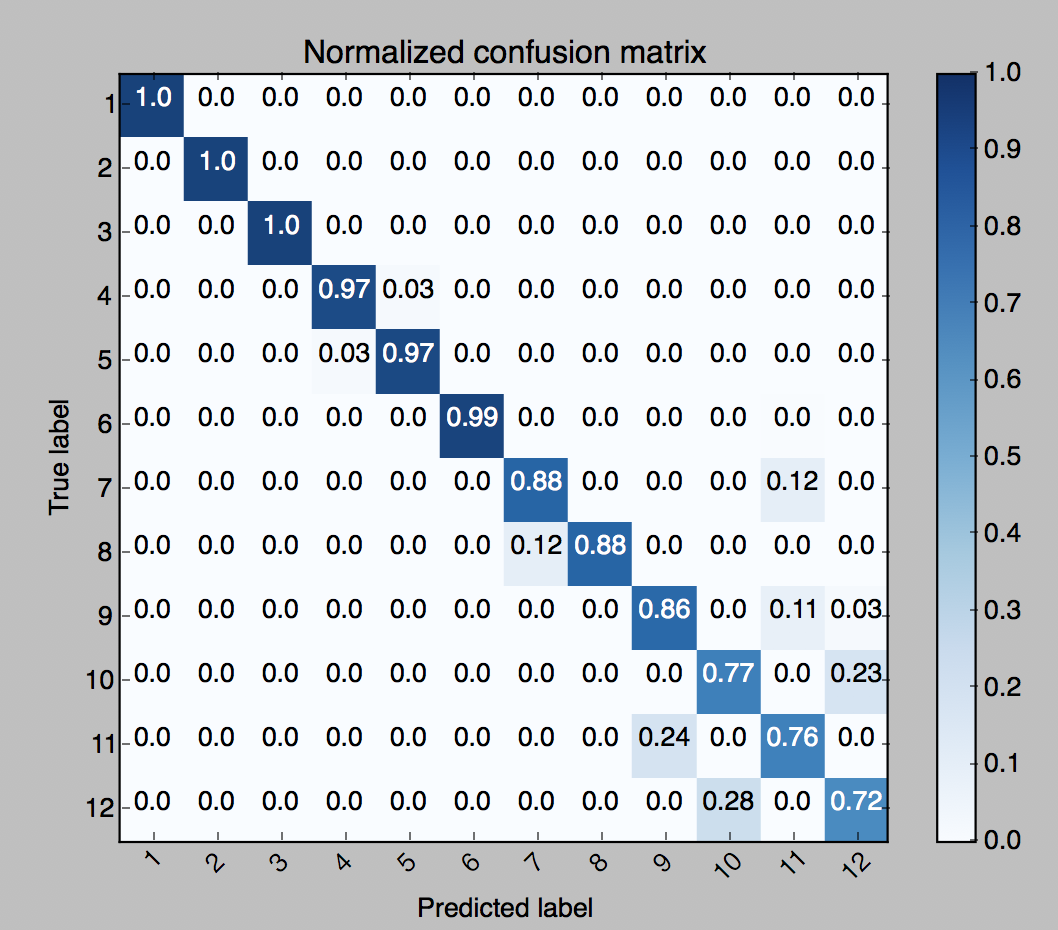
\includegraphics[width=0.5\textwidth]{fourthN.png}
\\

\section{Conclusions from the experimentation}

\subsection{Results}

As the results show SVM with specific parameters was the most correct algorithm, with an average of 98.08\% correct. There was an issue with lack of data on the last six classes, leading to very high correctness for the first six then a fairly obvious drop off on the last six.

\subsection{Ethics}

The ethics of having this data with the participants full knowledge and permission is perfectly acceptable, this can change however if consent is not given. If this data was used by any third parties to use in any activities such as marketing or tracking, this is unacceptable. This boundary can however be moved in the case of emergency fire and rescue needing the data for a search and rescue in the case of a fire or earthquake. 

\section{References}

Toby Breckon - www.github.com/tobybreckon/python-example-ml

%%% End document
\end{document}